\documentclass[a4paper, twocolumn, 10pt]{article}

\usepackage[english]{babel}
\usepackage[latin1]{inputenc}
\usepackage[T1]{fontenc}

\usepackage{float} % For controlling figure positions

\usepackage{amsthm} % For using \begin{proof}...
\usepackage{amsfonts}
\usepackage{amssymb}
\usepackage{amsmath}
\usepackage{fancybox}
\usepackage{color}
\usepackage{cite}
\usepackage{url}

\usepackage{algorithm}
\usepackage[noend]{algpseudocode}
\usepackage{program}

\usepackage{authblk}

\title{Neutral competition promotes chaos \\ {\color{red} Draft}}
\author[1]{Pablo Rodr�guez-S�nchez \thanks{pablo.rodriguezsanchez@wur.nl}}
\author[1]{Egbert van Nes \thanks{egbert.vannes@wur.nl}}
\author[1]{Marten Scheffer \thanks{marten.scheffer@wur.nl}}

\affil[1]{Department of Aquatic Ecology, Wageningen University, The Netherlands}

\usepackage{graphicx}
\graphicspath{ {../img/} }

\begin{document}

%\title{}
%\author{Pablo Rodr�guez-S�nchez \\ \\ Wageningen University}
%\author{Pablo Rodr�guez-S�nchez \\ \\ pablo.rodriguez.sanchez@gmail.com \\ \\ https://sites.google.com/site/pablorodriguezsanchez/}
%\date{\today}

\maketitle

%\begin{center}
%	\label{fig:QR}
%	\includegraphics[scale=0.4]{QR_main.png}
%\end{center}

\begin{abstract}
An increase in the neutrality of the competition at the prey's trophic level in a two-level food web rises the chances of chaotic behaviour in the long term.

\paragraph{}
\textit{Keywords}: population dynamics, competition models, chaos.
\end{abstract}

\tableofcontents

\section{Introduction}
\label{sec:Introduction}
The biodiversity paradox, that can be carelessly rephrased as \textit{Why are there so many species?}, is one of the main problems in theoretical ecology. The paradox consists in the contradiction between the competitive exclusion principle and the observed biodiversity. In the current state of the art, there are several alternative hypotheses for dealing with this problem. Two of these hypotheses are: \textit{a. Hubbell's neutral competition theory} \cite{Hubbell2001} and \textit{b. Ecosystems as non-equilibrium systems}. {\color{red} More references about the controversy are probably advisable here}. 

\paragraph{}
Hubbell's neutral competition theory, despite its counter-intuitive foundations, has been successfully applied to populations of rainforest trees. {\color{red} I don't see the relationship of Hubbell's theory with the biodiversity paradox}.

\paragraph{}
If ecosystems are proven to be non-equilibrium systems, the biodiversity paradox will be automatically solved. Despite the population of a particular species can vary greatly in time, the overall picture will contain a large mix of species at each and every time. From the mathematical point of view, non-equilibrium systems have cyclic or chaotic attractors associated with their dynamics. The analysis of this attractors is a well known method, used often in physics and climate sciences.

\paragraph{}
Our simulations show that the likelihood of chaos in a competition model increases with neutrality at the competitors' trophic level, so both hypotheses are not completely independent. {\color{red} This should be at the end of the introduction?, or just a the conclusions section?}

\paragraph{}

{\color{red} A more detailed overview of the competing hypotheses and/or of another natural phenomena explained by chaos can be an interesting introduction.}

\section{Model description}
\label{sec:Model}
We will use a generalized Rosenzweig-MacArthur predator-prey model \cite{Rosenzweig1963, Scheffer2004} with two trophic levels. It will be composed of $ n $ preys and $ N $ predators.

\begin{figure}[h]
	\begin{center}
		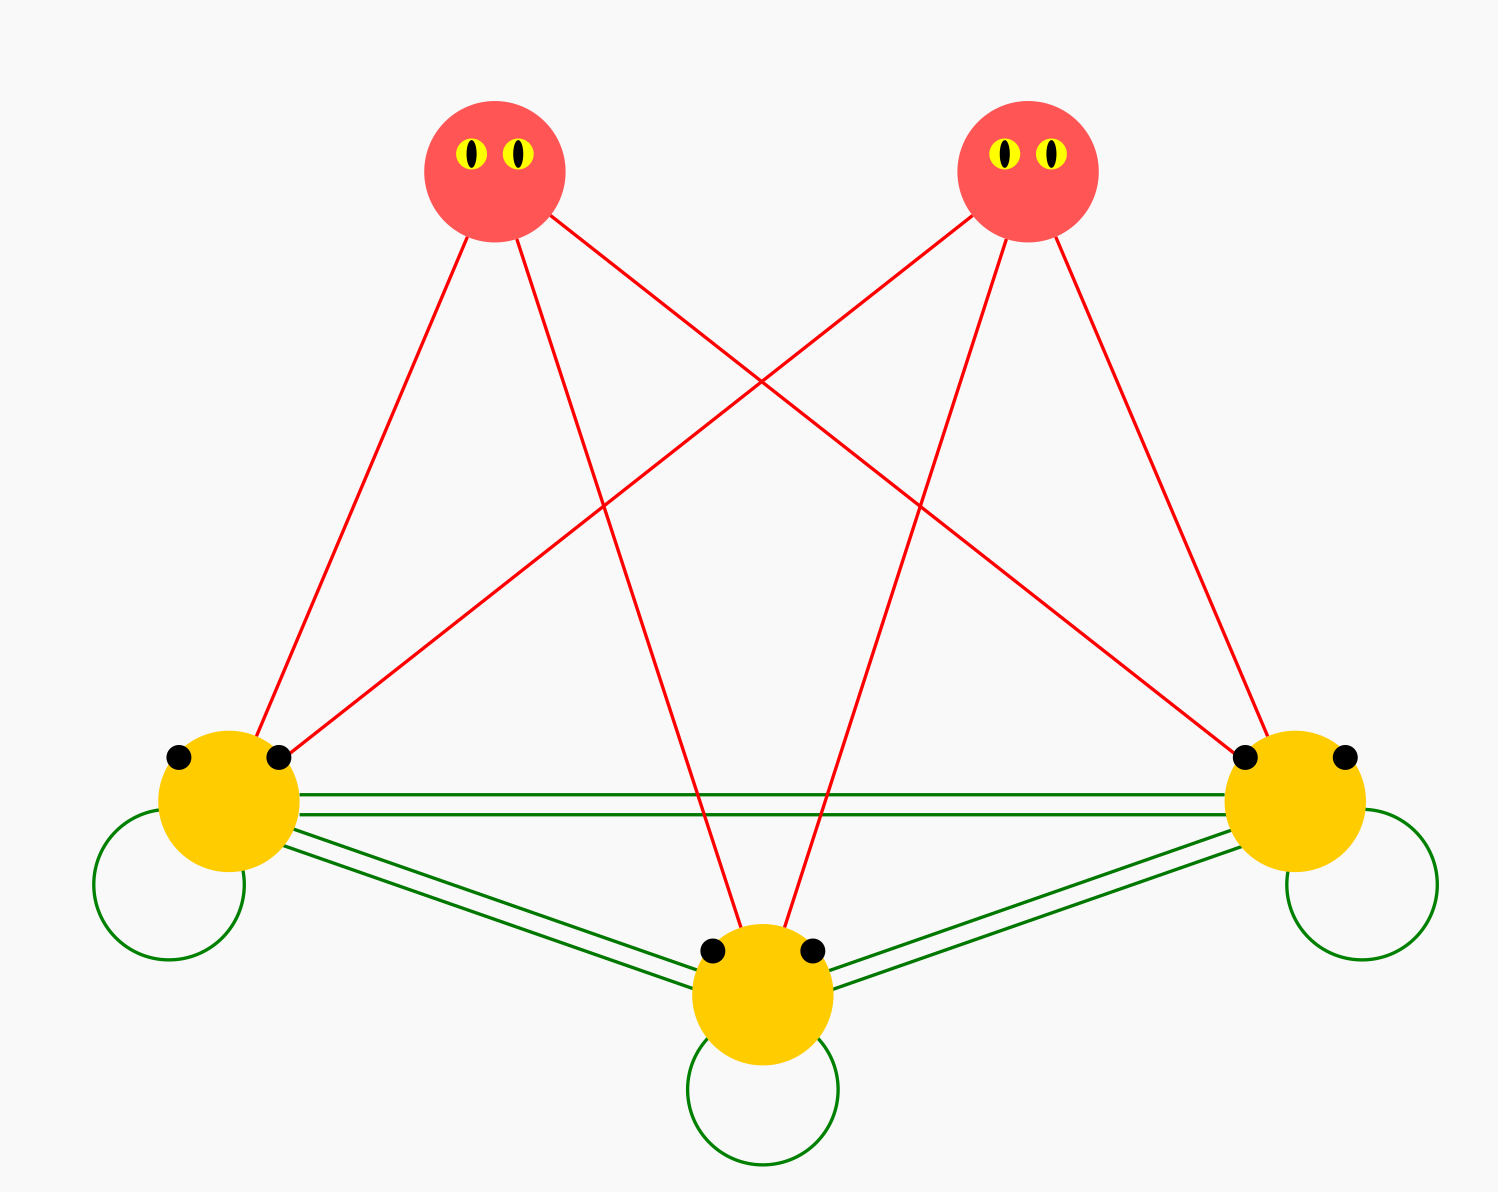
\includegraphics[width=0.9\columnwidth]{net.png}
	\end{center}
	\caption{Example with $2$ predators and $3$ preys. Each one of the red links represents a palatability coefficient (coded in the matrix $ S $). Each green link represents a competition coefficient (coded in matrix $ A $). The closed green loops are related with carrying capacity (diagonal elements of $ A $) interpreted here as intra-species competition.}
	\label{fig:Network}
\end{figure}

We will use $ p_i $ for accounting the size of the population of prey $ i $, and $ P_j $ for the population of predator $ j $. When it is not explicitly stated, $ i $ will run from $ 1 $ to $ n $, and $ j $ from $ 1 $ to $ N $. The preys compete among themselves, and the predators don't. The preys competition doesn't need to be necessarily symmetrical. The predators eat all kind of preys (see figure \ref{fig:Network}), but find some of them preferable than others.

\paragraph{} 
The dynamics can be described as a $ n + N $ dimensional system of ordinary, autonomous differential equations. The overall structure looks like:

\begin{displaymath}
\label{eq:EquationInPseudocode}
	\begin{cases}
	\frac{d}{dt} \left( prey \right) = Growth  - Predation + Immigration \\
	\frac{d}{dt} \left( Pred \right) = Feeding - Death \\
	\end{cases}
\end{displaymath}

The growth term is modelled as a multispecies logistic growth. The strength of the competition is given by $ A_{ik} $. Those coefficients can be arranged as a $ n \times n $ matrix. So, for prey $ i $, we have:

\begin{equation}
\label{eq:Growth-Competition}
\resizebox{.8 \columnwidth}{!}
{
$ Growth_i  = r p_i \left( 1 - \frac{1}{K} \sum_{k=1}^n A_{ik} \cdot p_k \right) $
}
\end{equation}

The palatability of each prey species is given by $ S_{ij} $. Those coefficients can be arranged as a $ N \times n $ matrix. Being a multispecies model, we can define the auxiliary variable $ V_j $ as a sum of the prey's populations weighted by the palatability coefficients. Biologically, this represents the overall composition of the "menu" of predator $ j $:

\begin{eqnarray}
\label{eq:AuxiliaryVectors}
	V_j \equiv \sum_{k=1}^n S_{jk} \cdot p_k
\end{eqnarray}

We hypothesize that the feeding term will be linear in $ P_j $, and have a Holling type II functional response on $ V_j $ in order to account for predator satiation:

\begin{equation}
\label{eq:Feeding}
	Feeding_j =  e g P_j F_{2}(V_j; H) = e g P_j \frac{V_j}{V_j + H}
\end{equation}

$ e $ represents the assimilation efficiency of the predation, that is, it regulates the biomass exchange between predator and prey. Thus, the effect of predator $ j $ on all prey's populations is given by $ Feeding_j/e $. Knowing this, we can sum the effect of all predators in the species $ i $ as follows:

\begin{equation}
\label{eq:Predation}
Predation_i = g p_i \sum_{k=1}^N S_{ki} \cdot \frac{P_k}{V_k+H} \equiv gp_iR_i
\end{equation}

Where for convenience, we have defined the auxiliary function $ R_i $ as a summary of this effect of all predators on prey $ i $:

\begin{equation}
\label{eq:PredationAux}
R_i(P_1, ..., P_N, V_k; S) \equiv \sum_{k=1}^N S_{ki} \cdot \frac{P_k}{V_k+H}
\end{equation}

Putting all together, the dynamical system reads:

\begin{eqnarray}
\label{eq:SystemUnderStudy}
	\begin{cases}
	\dot{p_i} = r p_i \left( 1 - \frac{1}{K} \sum_{k=1}^n A_{ik} \cdot p_k \right) - g p_i R_i + f
	\\ 
	\dot{P_j} = e g P_j \frac{V_j}{V_j + H} - l P_j
	\end{cases}
\end{eqnarray}

Depending on the parameters and the initial conditions, this system can give rise to four types of behaviour on the long term, each of them corresponding with a different type of attractor (see figure \ref{fig:TimeSeries}). The easier one, corresponding to a stable point attractor, gives rise to a constant species composition in the system. Cyclic attractors, that can be sub-classified as simple or complex, give rise to periodic behaviour in the species composition. Finally, chaotic attractors, makes the species composition keep evolving without stabilising nor giving rise to periodicity.

\begin{figure}
	\begin{center}
		\includegraphics[width=1\columnwidth]{time_series.png}
	\end{center}
	\caption{Time series of the species composition. First figure shows an stable attractor. The second one, a simple cyclic attractor. The third corresponds to a complex cyclic attractor. The last one shows a chaotic attractor}
	\label{fig:TimeSeries}
\end{figure}

\subsection{Parameterization}
\label{subsec:Parameterization}
Taking \cite{Dakos2009} as reference, we will use the following values for our parameters:

\begin{figure}[H]
	\begin{center}
		\resizebox{\columnwidth}{!}{%
		\begin{tabular}{|c|c|c|c|}
			\hline
			\textbf{Symbol} & \textbf{Interpretation} & \textbf{Value} & \textbf{Dimensions} \\
			\hline
			$r$ & Growth rate & $0.5$ & $T^{-1}$ \\
			\hline
			$g$ & Predation rate & $0.4$ & $T^{-1}$\\
			\hline
			$l$ & Loss rate & $0.15$ & $T^{-1}$\\
			\hline
			$K$ & Carrying capacity & $1$ & $M$ \\
			\hline
			$H$ & Half-saturation biomass & $2$ & $M$\\
			\hline
			$f$ & Immigration rate & $10^{-5}$ & $M \cdot T^{-1}$\\
		    \hline
			$e$ & Assimilation efficiency & $0.6$ & $1$\\
		    \hline
		    $S$ & $ N \times n $ palatability matrix & $S_{ij} \sim (0,1)$ & $1$\\
		    \hline
   		    $A$ & $ n \times n $ competition matrix & See section \ref{subsec:CompetitionParameter} & $1$\\
		    \hline
		\end{tabular}}
	\end{center}
	\caption{Values and meanings of the parameters used}
	\label{tab:Parameters}
\end{figure}

As explained in section \ref{subsec:ParameterReduction}, this system allows parameter reduction.

\section{Methodology}
\label{sec:Methodology}

Our aim is to analyse the behaviour of the system described in equation \ref{eq:SystemUnderStudy} for increasingly more neutral competition interactions. In order to accomplish this, we define in section \ref{subsec:CompetitionParameter} a \textit{competition parameter} ($ \epsilon $), a single parameter that controls the overall neutrality of the competition interaction.

\paragraph{}
For different values of neutrality (i.e., of $ \epsilon $), we'll estimate the probability of the system developing a chaotic attractor (see section \ref{subsec:DetectionOfChaos}).

\paragraph{}
Due to the complexity of the system, we have faced the problem as a numerical simulation (see sections \ref{subsec:Software} and \ref{subsec:NumericalExperiment}). As well, and for the sake of reproducibility, we provide a \textit{GitHub} link to the scripts used for analysis. {\color{red}Discuss with Egbert and Marten about which code repository use}

\subsection{Competition parameter}
\label{subsec:CompetitionParameter}
In order to control easily the neutrality of the competition, we introduce the competition parameter $ \epsilon $. This dimensionless parameter will allow us to vary continuously from interactions where intra-specific competition is stronger that inter-specific (for $ \epsilon < 0 $) to the opposite case (for $ \epsilon > 0$). The border between both cases (i.e. $ \epsilon = 0 $) represents neutral competition (see figure \ref{tab:CompetitionParameter}).

\paragraph{}

In order to accomplish this, we build our competition matrix using:

\begin{eqnarray}
\label{eq:NeutralityParameter}
	A(\epsilon) = A_0 + \epsilon \cdot W
\end{eqnarray}

Where $ A_0 $ is a totally neutral competition matrix (i.e., all its elements equal $ 1 $) and $ W $ is a random matrix whose non-diagonal elements have been drawn from a uniform distribution bounded to the interval $ [0, 1] $, and whose diagonal elements are zero. This way, we make sure that the diagonal elements of $ A $ are $ 1 $ in all cases (see figure \ref{tab:CompetitionParameter}).

\begin{figure}[H]
	\begin{center}
		\resizebox{\columnwidth}{!}{%
		\begin{tabular}{|c|c|c|}
			\hline 
			\textbf{Parameter value} & \textbf{Stronger competition} & \textbf{Example of competition matrix} \\
			\hline 
			$\epsilon < 0$ & Intra-specific & $ A = \begin{bmatrix} 1&.2&.3\\ .3&1&.4 \\ .5&.4&1\end{bmatrix} $ \\ 
			\hline 
			$\epsilon = 0$ & Neutral & $A = \begin{bmatrix} 1&1&1\\ 1&1&1 \\ 1&1&1\end{bmatrix}$ \\ 
			\hline 
			$\epsilon > 0$ & Inter-specific & $A = \begin{bmatrix} 1&1.7&1.6\\ 1.9&1&1.5 \\ 1.8&1.6&1\end{bmatrix}$ \\ 
			\hline 
		\end{tabular}}
	\end{center}
	\caption{Effect of the competition parameter on the competition matrix. Notice that the diagonal elements are always $ 1 $}	
	\label{tab:CompetitionParameter}
\end{figure}

\subsection{Software}
\label{subsec:Software}
All the subsequent analysis were performed using our software package GRIND for MATLAB\footnote{Freely available at \\ \url{http://www.sparcs-center.org/grind.html}}

\paragraph{} {\color{red}Publish code and add link}

\subsection{Numerical experiment}
\label{subsec:NumericalExperiment}

The objective is to estimate the probability of a chaotic attractor being reached as a function of the competition parameter ($ \epsilon $) controlling neutrality. In order to accomplish this task, we designed the following numerical experiment. It consists on repeating the following steps $ R $ times for each of the competition parameters drawn from the range $[-1,2]$:

\begin{enumerate}
	\item Use the competition parameter $\epsilon$ to generate a competition matrix $A$ (as described in section \ref{subsec:CompetitionParameter})
	\item \label{StartOfAnExperiment} Draw the rest of parameters and initial conditions from the ranges described in \cite{Dakos2009}, taken as uniform PDFs
	\item Determine numerically if the attractor generated by this conditions is chaotic or not (see section \ref{subsec:DetectionOfChaos}), and store the value of the maximum Lyapunov exponent
	\item Go back to step (\ref{StartOfAnExperiment}) $R$ times
\end{enumerate}

For those more familiar with flow charts, figure \ref{fig:FlowChart} can be illuminating.

\begin{figure}[H]
	\begin{center}
		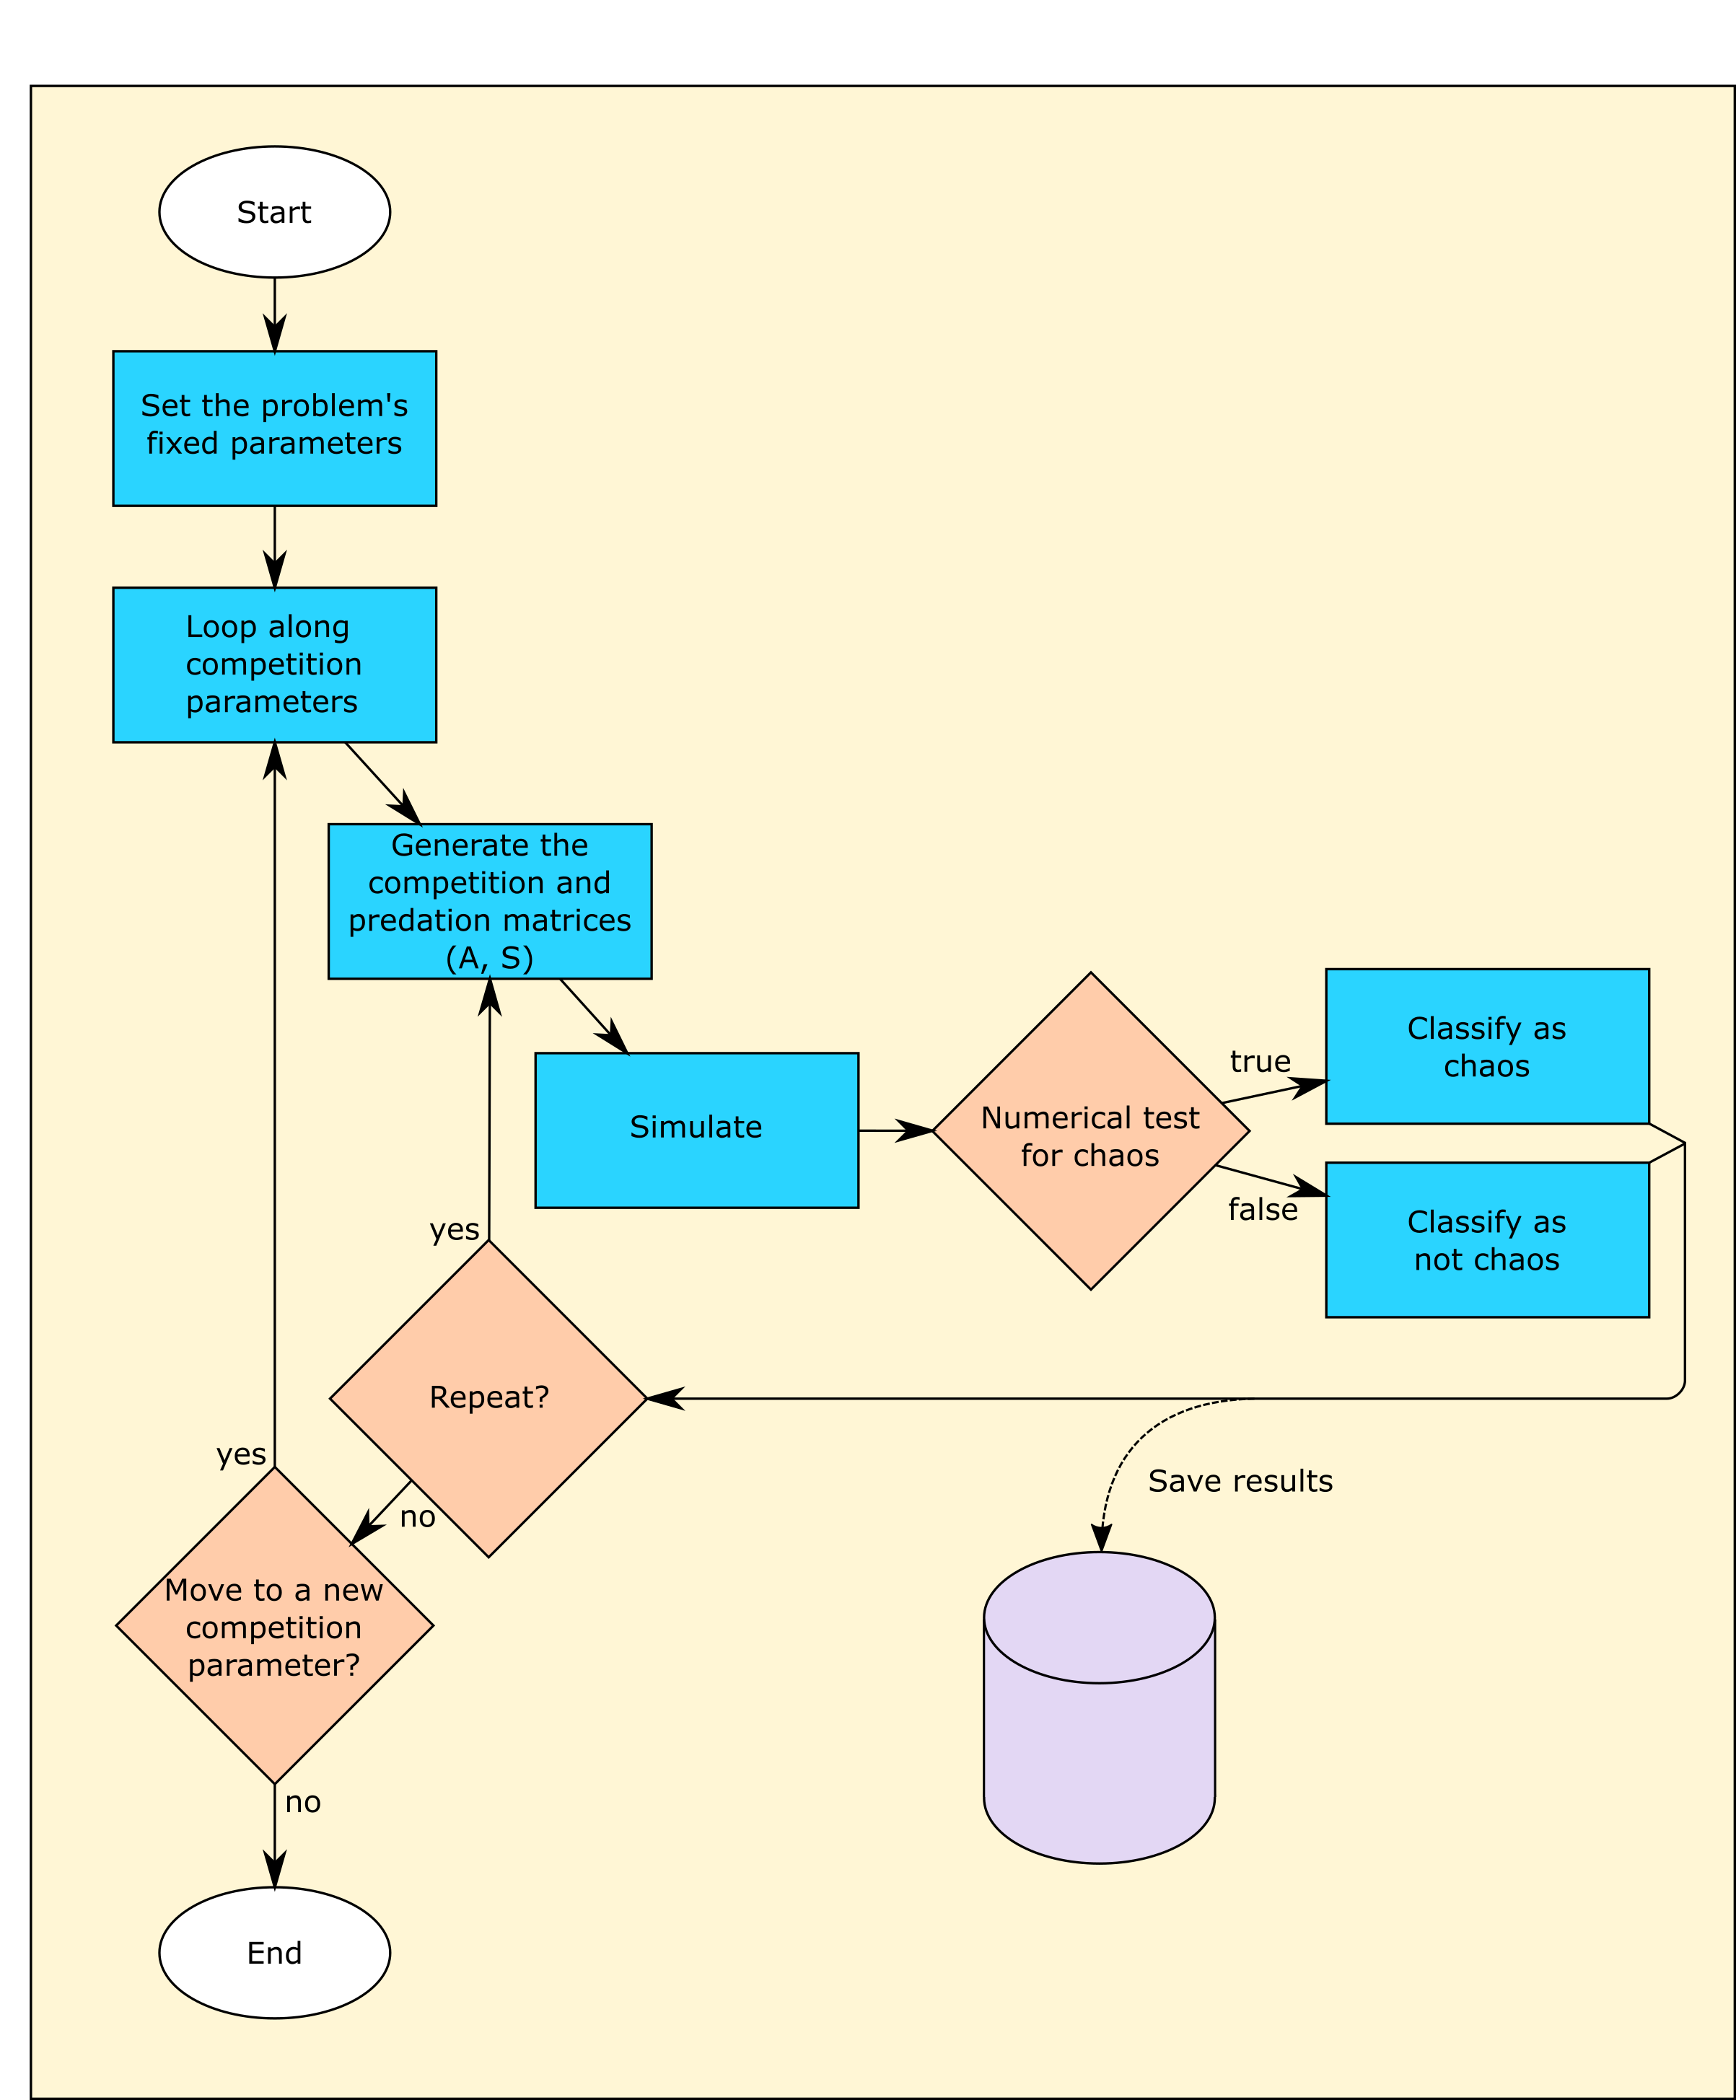
\includegraphics[width=0.9\columnwidth]{flow_chart.png}
	\end{center}
	\caption{Flow chart describing the numerical experiment}
	\label{fig:FlowChart}
\end{figure}

The outcome of the numerical experiment described above is a list of $ R $ maximum Lyapunov exponents per value of $ \epsilon $. This list can be used to estimate the probability of chaos for each value of $ \epsilon $ (see section \ref{subsec:DetectionOfChaos}).

\paragraph*{}
This numerical experiment can be repeated for different number of preys and predators ($n$ and $N$). {\color{red} Choose a fixed predator-prey ratio, keep it, and mention it here}

\subsection{Detection of chaos}
\label{subsec:DetectionOfChaos}
The procedure for classifying the attractors as chaotic or not is based in the analysis of Lyapunov exponents (see figure \ref{fig:FlowChart} and reference \cite{Strogatz1994}). More specifically, the procedure will be the following (see figure \ref{fig:FlowChart}):

\begin{enumerate}
	\item \label{GoToAttractor} Run the simulation for time enough, in order to guarantee that an attractor has been reached
	\item \label{RunInAttractor} Use the run in step \ref{GoToAttractor} as a starting point for a second, shorter run inside the attractor
	\item Use the run in step \ref{RunInAttractor} to compute numerically the principal Lyapunov exponent	
	\begin{itemize}
		\item If it's positive, classify the attractor as chaotic
		\item If it's negative, classify the attractor as non-chaotic
	\end{itemize}
\end{enumerate}

{\color{red} Big warning here: our method for detecting chaos sometimes gives false positives for complex cycles}

\paragraph{}
The probability of chaos can be estimated via the classical bayesian interpretation of probability, that is:

\begin{equation}
\label{eq:Probability}
	P(Chaos) \approx \frac{\#_{chaos}}{\#_{total}}
\end{equation}

\section{Results}
\label{sec:Results}

Plotting the probability of chaos against the competition parameter (see figures \ref{fig:Results} and \ref{fig:Contour}), we observe a clear maximum in the probability of chaos around $ \epsilon = 0 $, that is, for neutral competition at the prey's trophic level. The overall likelihood of chaos increases with dimensionality, but a maximum is still clearly appreciable for the neutral case.

\begin{figure}
	\begin{center}
		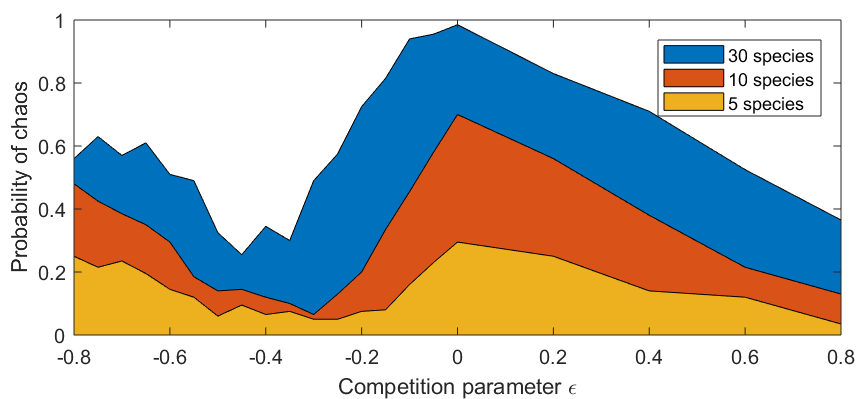
\includegraphics[width=0.9\columnwidth]{results.png}
	\end{center}
	\caption{Results for a low, medium and high dimensional system. The upper row represents the measured Lyapunov exponents, coloured in red if larger than zero, and in blue if smaller. The lower row represents the estimated probability of chaotic behaviour}
	\label{fig:Results}
\end{figure}

\begin{figure}
	\begin{center}
		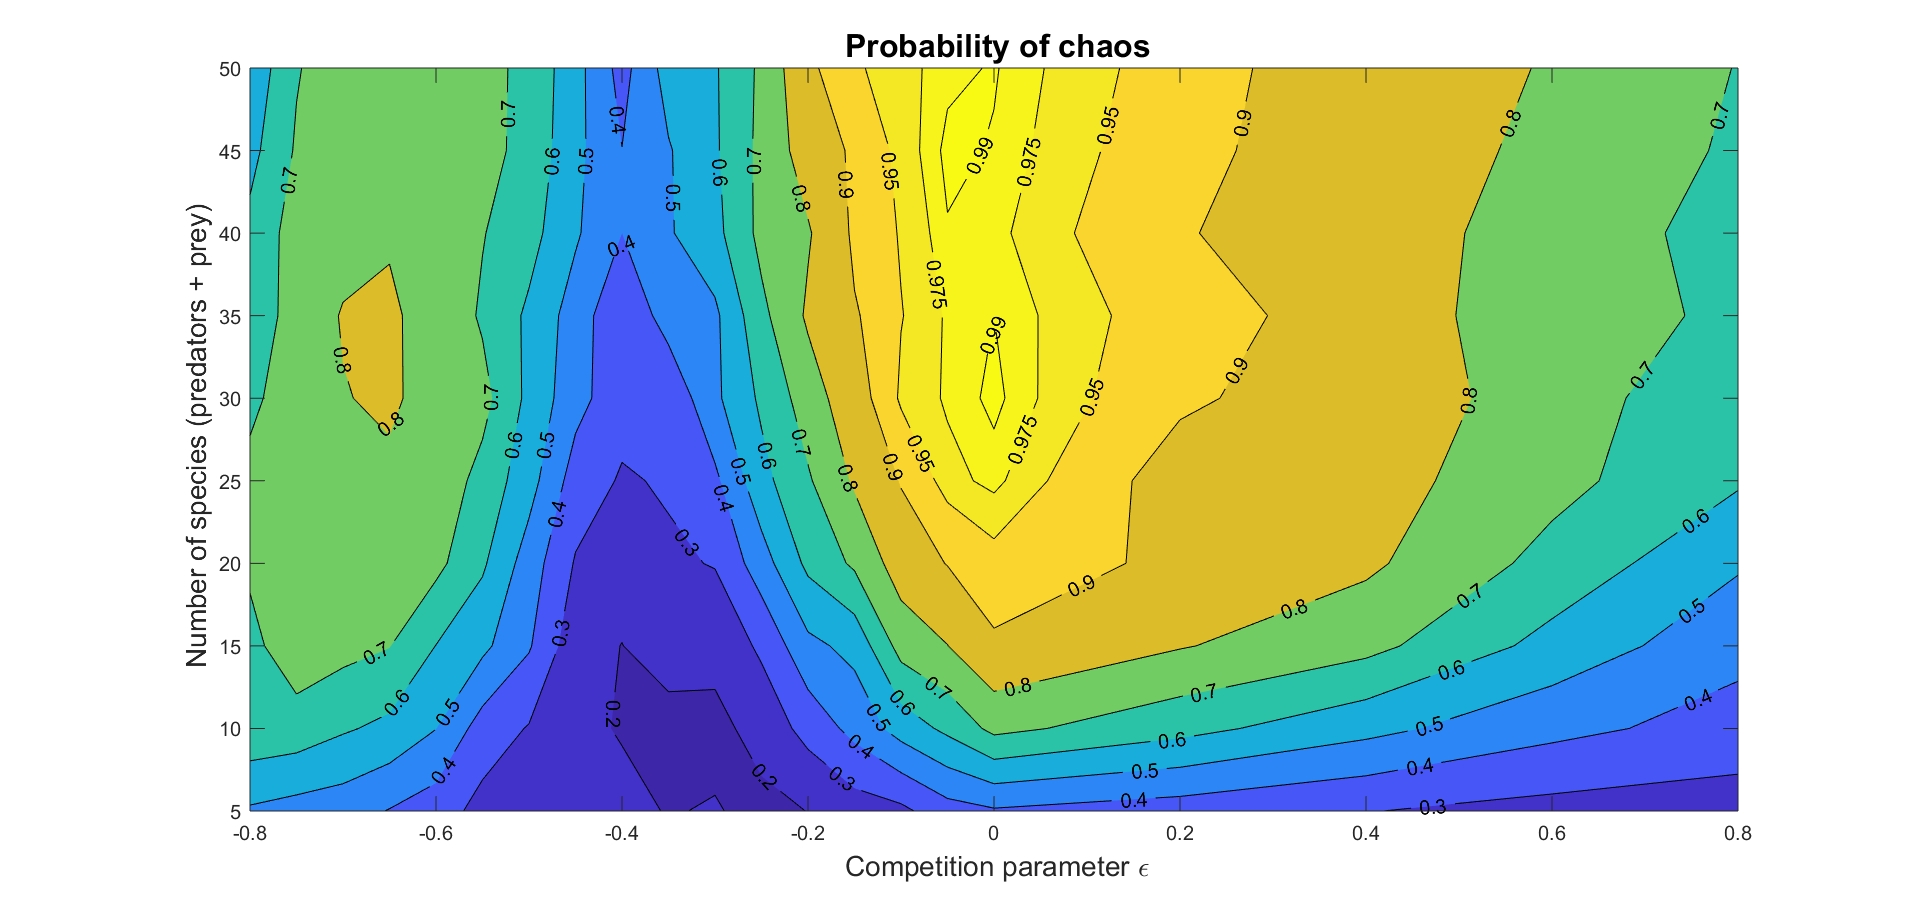
\includegraphics[width=1\columnwidth]{contour.png}
	\end{center}
	\caption{Contour map showing the probability of chaos for various competition parameters (horizontal axis) and prey populations (vertical axis). The predators' population is fixed as $ 2/3 $ of the prey's population, in order to control the overall size of the system with a single parameter. Notice that chaotic attractors appear more easily (i.e., for smaller systems) if the competition is neutral (i.e., $ \epsilon = 0 $)}
	\label{fig:Contour}
\end{figure}

\section{Conclusions}
\label{sec:Conclusions}

The fact that the overall likelihood of chaos increases with the amount of competing species, or equivalently, the system's dimensionality, is quite reasonable. Intuitively, we can understand this as increasing the available room for the formation of a complex chaotic attractor in the phase space.

\paragraph{}
Much more interesting and counterintuitive is the fact that neutrality, being a simplifying assumption (cf. section \ref{subsec:NeutralCompetition}), increases the likelihood of chaos, and therefore the complexity of the problem.

\paragraph{}
From the biological point of view, we show that the hypotheses mentioned at the introductory section \ref{sec:Introduction} are not completely independent. Maybe this can be a first step to reconcile both views.

\paragraph{}
{\color{red} Go deeper into the biological interpretation of the conclusion}

\section{Appendix}
\label{sec:Appendix}

\subsection{Neutral competition}
\label{subsec:NeutralCompetition}
If we drop everything but the competition part of our dynamics (see equation \ref{eq:SystemUnderStudySimplified}), we will find a system of equations $ n $ like the following:

\begin{eqnarray}
\label{eq:OnlyCompetition}
\dot{p_i} = p_i \left( 1 - \sum_{k=1}^n A_{ik} \cdot p_k \right)
\end{eqnarray}

In order to model a neutral competition, we should use the same competition coefficient for each species. That is, take $ A_{ik} = A $ for all $ i $ and $ k $, so:

\begin{eqnarray}
\label{eq:OnlyNeutralCompetition}
\dot{p_i} = p_i \left( 1 - A \sum_{k=1}^n p_k \right)
\end{eqnarray}

From equation \ref{eq:OnlyNeutralCompetition} we see that all species have exactly the same dynamical equation. This will make the nullclines to coincide at all points, so the equilibrium points will degenerate to equilibrium manifolds.

\begin{figure}[h]
	\begin{center}
		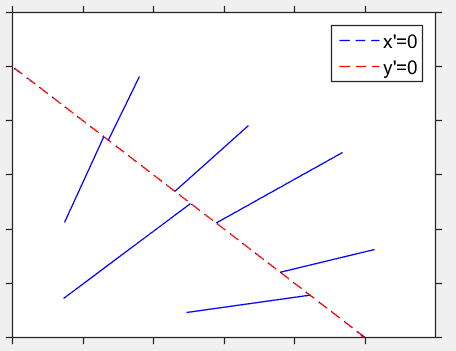
\includegraphics[width=0.9\columnwidth]{degenerate.png}
	\end{center}
	\caption{Example with $2$ prey under neutral competition. Both nullclines coincide point to point, giving rise to a higher dimensional equilibirium manifold (in this case, a straight line)}
	\label{fig:Neutral}
\end{figure}

This problem can be solved more easily noticing that, from the sole point of view of competition, the effect of neutrality is to fade out the differences between species, so the labels $ i $ distinguishing them become pointless. It is a good idea to sum up all the competing species into a single variable, that of total population of (indistinguishable) species, defined by:

\begin{eqnarray}
\label{eq:TotalPopulation}
	T(t) = \sum_{i=1}^n p_i(t)
\end{eqnarray}

It can be easily shown using equation \ref{eq:OnlyNeutralCompetition} that, as expected from the biological intuition, the dynamics of this new variable will follow the same differential equation as the individual species abundances:

\begin{eqnarray}
\label{eq:TotalPopulationDynamics}
	\dot T(t) = \sum_{i=1}^n \dot p_i(t) = T (1 - A T)
\end{eqnarray}

In our model, the predation interaction breaks this excess of symmetry, so we can still work with neutral competition as long as the predation is not neutral without facing problems of system degeneration.

\subsection{Parameter reduction}
\label{subsec:ParameterReduction}

The dynamical system \ref{eq:SystemUnderStudy} has $ n^2 + n \cdot N + 7 $ parameters. Choosing appropriate units and parameter combinations, this number can be reduced by $ 3 $:

\begin{itemize}
	\item By choosing an appropriate time scale $ \left( \tau = r t \right)$ we can get rid of $ r $
	\item $ K $ can be absorbed into $ A_{ij} $ $ \left( \frac{A_{ij}}{K} \rightarrow A_{ij}  \right) $ 
	\item $ H $ can be absorbed into $ S_{ij} $ $ \left( \frac{S_{ij}}{H} \rightarrow S_{ij}  \right) $
\end{itemize}

So, finally we have:

\begin{eqnarray}
\label{eq:SystemUnderStudySimplified}
	\begin{cases}
		\dot{p_i} = p_i \left( 1 - \sum_{k=1}^n A_{ik} \cdot p_k \right) - g p_i R_i + f
		\\
		\dot{P_j} = e g P_j \frac{V_j}{V_j + 1} - l P_j
	\end{cases}
\end{eqnarray}

with the $ n^2 + n \cdot N + 4 $ external parameters, namely:

\begin{figure}[H]
	\begin{center}
		\resizebox{\columnwidth}{!}{%
	    \begin{tabular}{ | c | c | c |}
	    \hline
	    \textbf{Parameter} & \textbf{Cardinal} & \textbf{Interpretation} \\ \hline
	    $ A_{ij} $ & $ n^2 $ & Competition between species $ i $ and $ j $\footnote{Also includes carrying capacity as "self" competition} \\ \hline
	    $ S_{ij} $ & $ n \cdot N $ & Palatability of the prey $ i $ for predator $ j $ \\ \hline
	    $ g $ & $ 1 $ & Effect of predation on prey \\ \hline
	    $ e $ & $ 1 $ & Predators' efficiency \\ \hline
	    $ f $ & $ 1 $ & Prey's immigration flow \\ \hline
	    $ l $ & $ 1 $ & Predators' death rate \\ \hline
	    \end{tabular}}
	\end{center}
	\caption{Parameters left after reduction}
	\label{tab:ParametersReduction}
\end{figure}

\subsection{Algorithm used}
\label{subsec:Algorithm}

The following pseudocode algorithm describes the whole procedure:

\makeatletter
\def\BState{\State\hskip-\ALG@thistlm}
\makeatother
\begin{algorithm}[H]
\caption{Pseudocode for the algorithm used}\label{Pseudocode}
	\begin{algorithmic}[1]
		\Procedure{Numerical experiment in pseudocode}{}
		\\
		\BState \emph{experiment design parameters}:
		\State $\textit{R} \gets \text{Number of repetitions}$
		\\
		\BState \emph{biological parameters}:
		\State $\textit{n} \gets \text{Prey's population}$
		\State $\textit{N} \gets \text{Predator's population}$
		\State $\textit{g} \gets \text{Effect of predation on prey}$
		\State $\textit{e} \gets \text{Predator's efficiency}$
		\State $\textit{f} \gets \text{Prey's immigration flow}$
		\State $\textit{l} \gets \text{Predator's death rate}$
		\\
		\BState \emph{loop}:
		\For{$\epsilon$ \textbf{in} $[-1,2]$}
		\State Draw a competition matrix $A$
		\State Draw a predation matrix $S$
		\State Draw random initial conditions
			\For{$i$ \textbf{in} $R$} 
			\State Compute dynamics
			\State Store maximum Lyapunov exponent $\lambda$
			\EndFor	
		\EndFor
		\\
		\BState \emph{results}:
		\State Return the lists $(\epsilon_i, \lambda_{i1}, ..., \lambda_{iR})$
		\EndProcedure
	\end{algorithmic}
\end{algorithm}

\section{Acknowledgements}
\label{sec:Acknowledgements}
We thank Jelle Lever for his useful comments and suggestions.

\color{red}
\section{To do}
\label{sec:ToDo}

\begin{itemize}
\item Send more details to the appendix?
\item Remove or improve the pseudocode algorithm
\item Clean and publish analysis code in \textit{GitHub}
\end{itemize}

Further ideas, for this or future papers:

\begin{itemize}
\item Neutrality in predation
\item Study symmetric competition with a parameter that controls symmetry
\item Neutrality increases symmetry as well. May this be related with the fact that, as said in \cite{Scheffer2004}, \textit{"symmetry in competition strongly promotes multiplicity of attractors"}
\end{itemize}


\color{black}
\clearpage
\bibliography{library}
\bibliographystyle{ieeetr}
%\bibliographystyle{apalike}

%\listoftables
\listoffigures

\end{document}
